\documentclass[9pt,twocolumn,twoside]{pnas-new}
% Use the lineno option to display guide line numbers if required.
% Note that the use of elements such as single-column equations
% may affect the guide line number alignment.

\usepackage{subcaption}
\usepackage{breqn}

% the follow ing causes latex to not wait interactively
\nonstopmode

\setboolean{displaywatermark}{false}

\templatetype{pnasresearcharticle} % Choose template 
% {pnasresearcharticle} = Template for a two-column research article
% {pnasmathematics} = Template for a one-column mathematics article
% {pnasinvited} = Template for a PNAS invited submission

\title{Dynein walks like an Imperial AT-ST}

% Use letters for affiliations, numbers to show equal authorship (if applicable) and to indicate the corresponding author
\author[a,c,1]{Author One}

\affil[a]{Oregon State University}

% Please give the surname of the lead author for the running footer
\leadauthor{Lead author last name} 

% Please include corresponding author, author contribution and author declaration information
\authorcontributions{Please provide details of author contributions here.}
\authordeclaration{Please declare any conflict of interest here.}
\equalauthors{\textsuperscript{1}A.O.(Author One) and A.T. (Author Two) contributed equally to this work (remove if not applicable).}
\correspondingauthor{\textsuperscript{2}To whom correspondence should be addressed. E-mail: author.two\@email.com}

% Keywords are not mandatory, but authors are strongly encouraged to provide them. If provided, please include two to five keywords, separated by the pipe symbol, e.g:
\keywords{dynein $|$ Brownian dynamics $|$ powerstroke $|$ modeling} 

\begin{abstract}
Please provide an abstract of no more than 250 words in a single paragraph. Abstracts should explain to the general reader the major contributions of the article. References in the abstract must be cited in full within the abstract itself and cited in the text.
\end{abstract}

\dates{This manuscript was compiled on \today}
\doi{\url{www.pnas.org/cgi/doi/10.1073/pnas.XXXXXXXXXX}}

\input{../../data/paper_params.tex}

\begin{document}

% Optional adjustment to line up main text (after abstract) of first page with line numbers, when using both lineno and twocolumn options.
% You should only change this length when you've finalised the article contents.
\verticaladjustment{-2pt}

\maketitle
\thispagestyle{firststyle}
\ifthenelse{\boolean{shortarticle}}{\ifthenelse{\boolean{singlecolumn}}{\abscontentformatted}{\abscontent}}{}

\dropcap{D}ynein is a motor protein used to generate directed force in cells. The protein is a homodimer which binds to cellular filaments known as microtubules (MTs). Each monomer has several ATPase domains arranged in a larger globular domain known as the ``head''. This head is the site which hydrolyzes ATP and undergoes the conformational changes responsible for dynein's step. The head is attached via a long chain to the microtubule binding domain (MTBD). Dynein is an interesting structure in that it manages to coordinate ATPase chemistry at its head with MT-releasing chemistry at its MTBD, some 20nm away \cite{mt-atp-coupling}. The head has a long tail domain coming off it, which eventually dimerizes to the other monomer.\\

Dynein is unique in that it has a widely varied step size. Dynein's average step is 8 \textit{nm} in the forwards direction, but it is capable of taking 32 \textit{nm} steps in the forwards and reverse directions \cite{weihongpaper} \cite{yildizpaper}. This stochastic, varied stepping is contrasted with the much more regular 8 \textit{nm} step size of kinesin, another bipedal motor protein \cite{kinesin-step-size}. It has been suggested that the long separation between dynein's MTBD and dimerization sites facilitates larger diffusive searches, allowing dynein to take larger steps than kinesin \cite{cargotransport}.\\

A simple explanation for dynein's stepping pattern can be given based on only a few facts about the protein. It is known that on treatment with ATP, the tail-head-MTBD angle of a dynein monomer alters, moving the MTBD closer to the tail \cite{carteradpprimed} \cite{burgess-paper}. It is also known that the nucleotide state of the head communicates with the MTBD. ATP binding at a head ATPase shifts the MTBD from a strong to weak MT-bound state. And vice-versa, whether the MTBD is bound or unbound from the MT changes the ATPase rate at the head. From this it is possible to infer a simple model for the dynein stepping cycle. This model, known as the mechanochemical cycle \cite{cianfroccoreview}, has dynein unbind MT, kick forward, diffuse to the next MT binding site, rebind MT, then repeat. Whether a model this simple can explain dynein's behavior needs to be tested.\\

There are many relevant details about dynein which this simple model doesn't account for. Dynein is known to have low interhead communication at low separation, but to have a tension-gated stepping pattern at high separations \cite{yildizpaper}. It is also suggested that dynein's MTBD doesn't conduct an undirected search for its next MT binding site, but rather is guided by long-range electrostatic interactions from each MT binding site \cite{longrangemt}. Dynein has several cofactors which alter its dynamics. For example, the motor's stall force is tripled when exposed to dynactin and Bic2D \cite{yildizdynactin}. This is odd, since the dynactin- and Bic2D-binding site on dynein is on the tail, far from the motor heads. Many of these details suggest a complicated picture of dynein motility than a simple forward kick and pull mechanism.\\

Several computational models have been created to explain dynein's motility. \textit{Imamula et. al.} define a chemical transition model which defines all the MT- and nucleotide-bound states dynein goes through as it walks \cite{imamulamodel}. \textit{Sarlah et. al} simulate a model obeying rate constants from \textit{Imamula}, and replicate dynein's stepping trajectory \cite{sarlahmodel}. \textit{Zheng} uses normal mode analysis to simulate the dynein motor's transition from pre to post-powerstroke \cite{normalmodes}. To our knowledge, no computational model exists which takes into account the microscopic dynamics of protein-water interactions to test whether diffusion is enough for dynein motility. Here we show how a simple Brownian dynamics model can be used to test the mechanochemical cycle picture of dynein processivity.\\

\section*{Model}

%% Figure X.1 - poststroke
%% FIgure X.2 - prestroke
%% Figure X.A: Model of the protein superimposed over cryo-EM data (with length data)
%% Figure X.B: Cryo-EM visualizations of how we get equilibrium angles
%% Add rod vectors connecting each domain

\begin{figure}[tbhp]
\centering
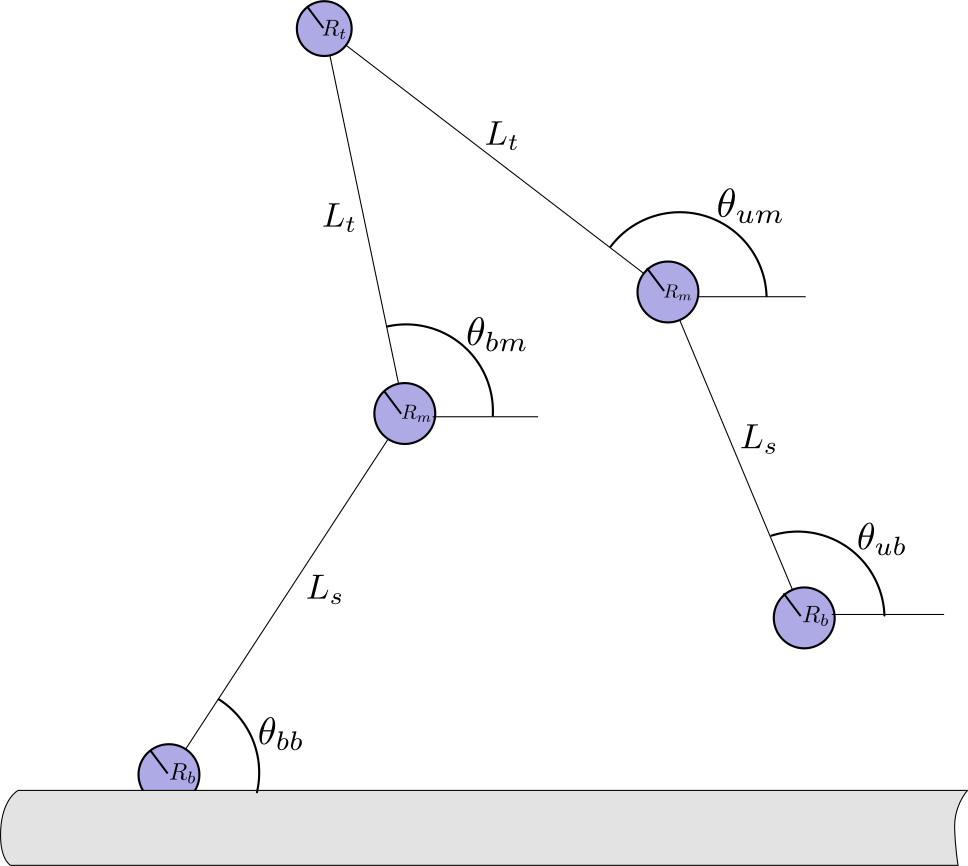
\includegraphics[width=0.49\linewidth]{figures/onebound-cartoon.pdf}%
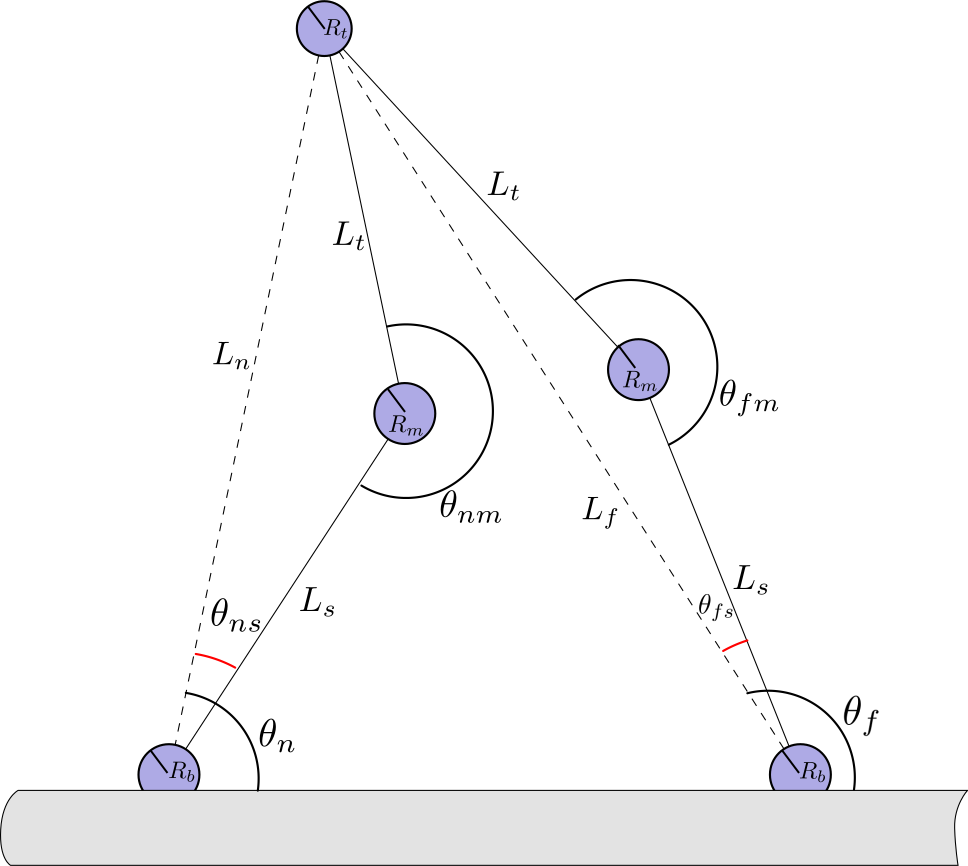
\includegraphics[width=0.49\linewidth]{figures/bothbound-cartoon.pdf}
\caption{}
\end{figure}

\begin{figure}[tbhp]
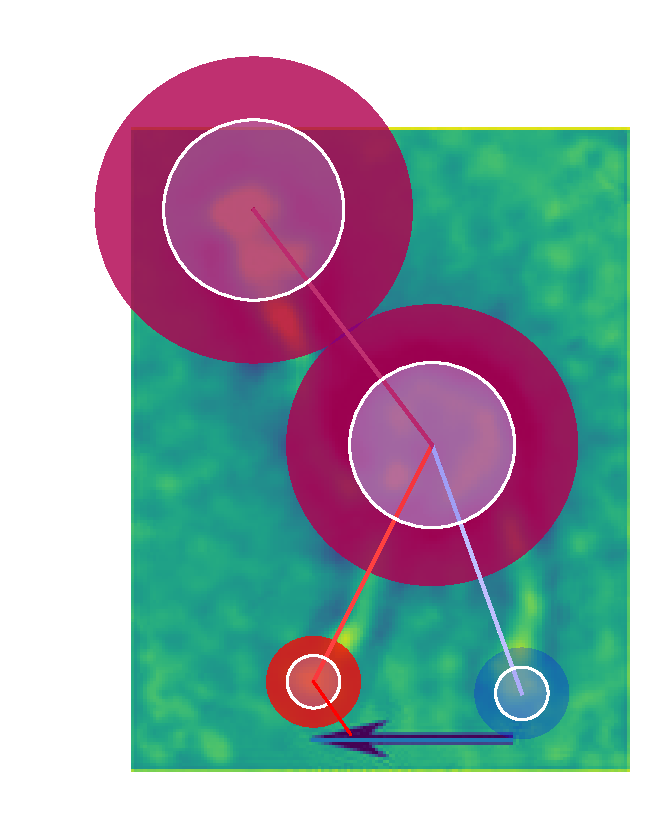
\includegraphics[width=0.4\linewidth]{../../plots/burgess-model-figure.pdf}%
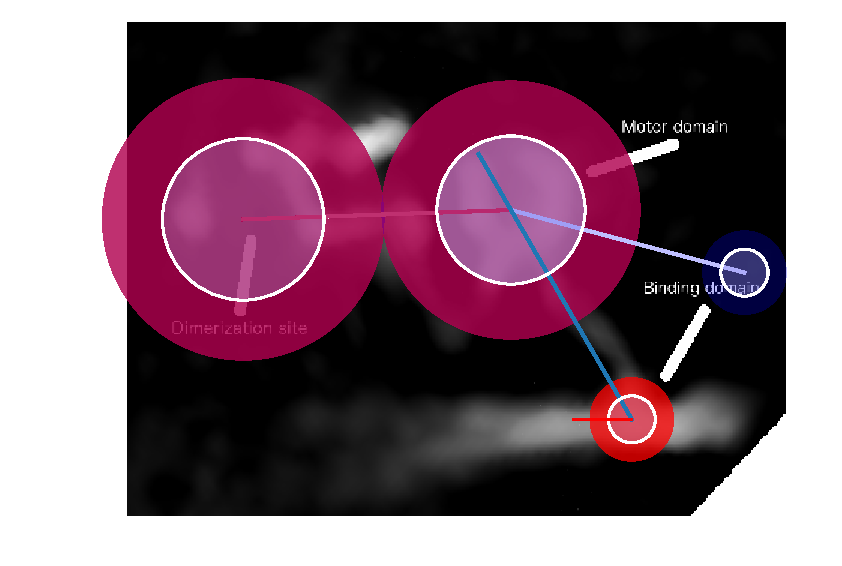
\includegraphics[width=0.6\linewidth]{../../plots/grotjahn-model-figure.pdf}%
%% 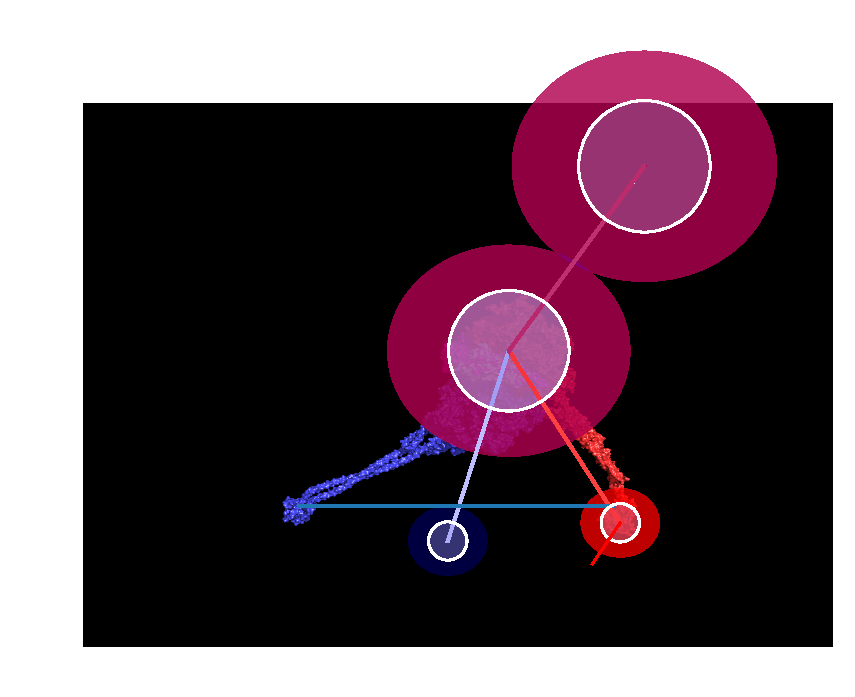
\includegraphics[width=0.3\linewidth]{../../plots/crystal-model-figure.pdf}%
\caption{\textbf{Hinge model compared with dynein micrographs.} \textit{Left:} Model at equilibrium angles superimposed over an axonemal dynein c micrograph consisting of an apo and and ADP-Pi-bound dynein monomer \cite{burgess-paper}; axonemal and cytoplasmic dynein have comparable size and architecture \cite{dynein-c-paper}. \textit{Right:} Model at equilibrium superimposed over full-length dimerized dynein bound to accessory proteins, (map ID EMD-7000) \cite{grotjahn}. Left figure has a scale bar of 15nm, right 26.3nm between MTBD and AAA1 of motor domain.}
\label{fig:duration-length}
\end{figure}


%% \textit{Black bg:} Model superimposed over crystal structures of two monomers, pink being the ADP-Pi-bound cytoplasmic dynein-2 monomer from human (PDB ID 4RH7), yellow being an apo cytoplasmic dynein monomer from yeast (PDB ID 3VKH), docked together using linkers as a reference point. Orange indicates the linker region used to dock the two monomers. 

\subsection*{Elastic hinge model}~\\
Our model is designed to capture the course-grained dynamics of the dynein protein while remaining mathematically tractable. We capture the structure of the full dynein complex by treating the protein as a set of spheres connected by rigid rods. Geometric properties of the model, such as rod length $L_s$ and $L_t$, and sphere radii $R_b$, $R_m$ and $R_t$, are calculated from electron microscopy and crystallography data, as pictured in Fig X.A. Each sphere acts as a hinge, and the angle between connected rods, or the MT, is free to vary. The model is constrained to remain in the plane of the microtubule, so transverse motion is not allowed. The model exists in two states: one called the poststroke state with both binding domain positions constant, as in Figure X.1, and one called the prestroke state with one binding domain free to move, as in Figure X.2.

\begin{table}[tbhp]
\centering
\caption{Parameters used in model simulation.}
\label{tab:staticparams}
\begin{tabular}{lrrr}
Parameter & Model & Experimental & Source \\
\midrule
$c_b$ & $\cb \Delta G_{ATP}$ &  & \\
$c_m$ & $\cm \Delta G_{ATP}$ &  & \\
$c_t$ & $\ct \Delta G_{ATP}$ &  & \\
$k_b$ & $\kb s^{-1}$&  & \\
$k_{ub}$ & $\kub s^{-1}$ & & \\
$L_s$ & $\ls nm$ & 21nm & \cite{burgess-paper, 3vkh-cite, carter-paper}\\
$L_t$ & $\lt nm$ & 23nm & \cite{burgess-paper, 3vkh-cite, carter-paper}\\
$c$ & $\cexp$ & & \\
$\theta_b$ & $\eqb$ &  120 & \cite{leschziner} \\
$\theta_m^{\mbox{pre}}$ & $\eqmpre$ &  197 & \cite{burgess-paper}\\
$\theta_m^{\mbox{post}}$ & $\eqmpost$ & 242 & \cite{burgess-paper}\\
$\theta_t$ & $\eqt$ &  & \\
$R_t$ & $\radiust$ & 8nm & \cite{burgess-paper}\\
$R_m$ & $\radiusm$ & 11nm & \cite{burgess-paper}\\
$R_b$ & $\radiusb$ & 3.5nm & \cite{burgess-paper}\\

\bottomrule
\end{tabular}

%% \addtabletext{nomenclature for the TSs refers to the numbered species in the table.}
\end{table}

\subsection*{Model dynamics}~\\
The model experiences internal and external forces. The internal forces are due to elastic restoring forces for each hinge angle ($\left[\theta_{bb}, \theta_{bm}, \theta_{t}, \theta_{um},\right]$ for prestroke, $\left[\theta_{nb}, \theta_{nm}, \theta_{t}, \theta_{fm}, \theta_{fb},\right]$ for poststroke) compared to its equilibrium ($\left[\Theta_{bb}, \Theta_{bm}, \Theta_{t}, \Theta_{um},\right]$ for prestroke, $\left[\Theta_{nb}, \Theta_{nm}, \Theta_{t}, \Theta_{fm}, \Theta_{fb},\right]$ for postsroke). These equilibrium angles are determined from cryo-EM micrographs of ATP-Vi-bound and ADP-bound dynein monomers, indicated in Figure X.B.\\

The torque on each domain is given by:
%
\begin{equation}
  \vec{\tau}_{i} = c_i\left(\theta_{i}-\Theta_{i}\right)\hat{z}
\end{equation}
%
The external forces on the model are random Brownian forces $\vec{R_i} = R_i\hat{x} + R_i\hat{y}$, where $R_i$ is a Gaussian random variable with $\mu_R = 0$ and $\sigma^2_R = 2kbT\gamma_i/dt$, where drag factor $\gamma_i = 6\pi\nu R_i$ with dynamic viscosity $\nu$. Brownian dynamics is used to calculate the velocity on each domain, where velocity is given by:
%
\begin{dmath}
  \vec{v}_i = \gamma_i^{-1}\left(\frac{\vec{\tau}_{i-1}}{L_{i-1}}\left(\hat{z}\times\hat{r}_{i-1}\right)
  + \frac{\vec{\tau}_{i+1}}{L_{i+1}}\left(\hat{z}\times\hat{r}_{i+1}\right)
  - \vec{\tau}_{i}\left(\frac{\hat{z}\times\hat{r}_{i-1}}{L_{i-1}}+\frac{\hat{z}\times\hat{r}_{i+1}}{L_{i+1}}\right) + \vec{R_i}\right)
  \label{eq:motionequation}
\end{dmath}
%
\subsection*{Powerstroke model}~\\
The dynein powerstroke is the hypothetical process whereby a motor unbinds from the microtubule, undergoes a linker remodel which pushes the motor forward, binds to the microtubule, and undergoes the opposite linker remodel, pulling the rest of the motor forward in a ``powerstroke.'' Our model simplifies the powerstroke cycle by alternating between two states: a two-foot-bound post-powerstroke state similar to the apo dynein, and a one-foot-bound pre-powerstroke state similar to the post-hydrolysis ADP-Pi dynein. Our model captures the prestroke kick of the unbound MTBD through different motor hinge equilibrium angles, as calculated from Figure X.B. The larger prestroke motor hinge angle causes a forward diffusion of the unbound binding domain on transition to one-foot-bound, followed by another forward diffusion of the whole motor as the MTBD binds and transitions back to post-stroke hinge angles.\\

Dynein's MTBD unbinding dynamics are known to be tension-dependent, where at high interhead separations unbinding favors the lagging MTBD, but no preference between leading and lagging is seen for small interhead separations \cite{yildizpaper}. To capture this, the microtubule unbinding rate $k_{ub}$ takes into account absolute binding angle:
%
\begin{equation}
  k_{ub} = k_{ub}^0e^{-c\left(\theta_{xb}-\Theta{xb}\right)}
\end{equation}
%
where $k_{ub}^0$ is the default unbinding rate and $c$ the unbinding exponential factor. Each timestep unbinding occurs with probability $k_{ub}dt$. On unbinding, the both-foot-bound model transitions to a one-foot-bound model with identical domain positions, but new equilibrium hinge angles. Microtubule binding occurs with probability $k_{b}^0dt$ if the binding domain is within $D$ nm of the microtubule. On binding, the one-foot-bound model transitions to a both-feet-bound with identical domain positions, but with both MTBDs constrained on the microtubule.\\

\subsection*{Simulating the model}~\\
The model was simulated using Euler's method to time evolve Equation \ref{eq:motionequation} using a timestep $dt$, transitioning freely between the poststroke and prestroke states.

\section{Results}

%% \begin{figure}%[tbhp]
%% \centering
%% \includegraphics[width=\linewidth]{../../plots/stepping_analysis_paper.pdf}
%% \caption{Histogram of duration of steps taken by model.}
%% \label{fig:timehist}
%% \end{figure}

%% \begin{figure*}[tbhp]
%%   \begin{subfigure}{0.5\textwidth}
%%     \centering
%%     \includegraphics[width=\linewidth]{../../plots/paper_static_step_length_histogram}
%%   \end{subfigure}%
%%   \begin{subfigure}{0.5\textwidth}
%%     \centering
%%     \includegraphics[width=\linewidth]{../../plots/paper_exponential_step_length_histogram}
%%   \end{subfigure}
%%   \begin{subfigure}{0.5\textwidth}
%%     \centering
%%     \includegraphics[width=\linewidth]{../../plots/paper_static_displacement_histogram}
%%   \end{subfigure}%
%%   \begin{subfigure}{0.5\textwidth}
%%     \centering
%%     \includegraphics[width=\linewidth]{../../plots/paper_exponential_displacement_histogram}
%%   \end{subfigure}
%%   \begin{subfigure}{0.5\textwidth}
%%     \centering
%%     \includegraphics[width=\linewidth]{../../plots/paper_static_displacement_vs_step_length}
%%     \subcaption{Static unbinding rate}
%%   \end{subfigure}%
%%   \begin{subfigure}{0.5\textwidth}
%%     \centering
%%     \includegraphics[width=\linewidth]{../../plots/paper_exponential_displacement_vs_step_length}
%%     \subcaption{Exponential unbinding rate}
%%   \end{subfigure}
%% \caption{Stepping behavior of static and exponential models, with parameters shown in Table \ref{tab:staticparams}.}
%% \label{fig:lengthhist}
%% \end{figure*}

\begin{figure}[tbhp]
  \centering
  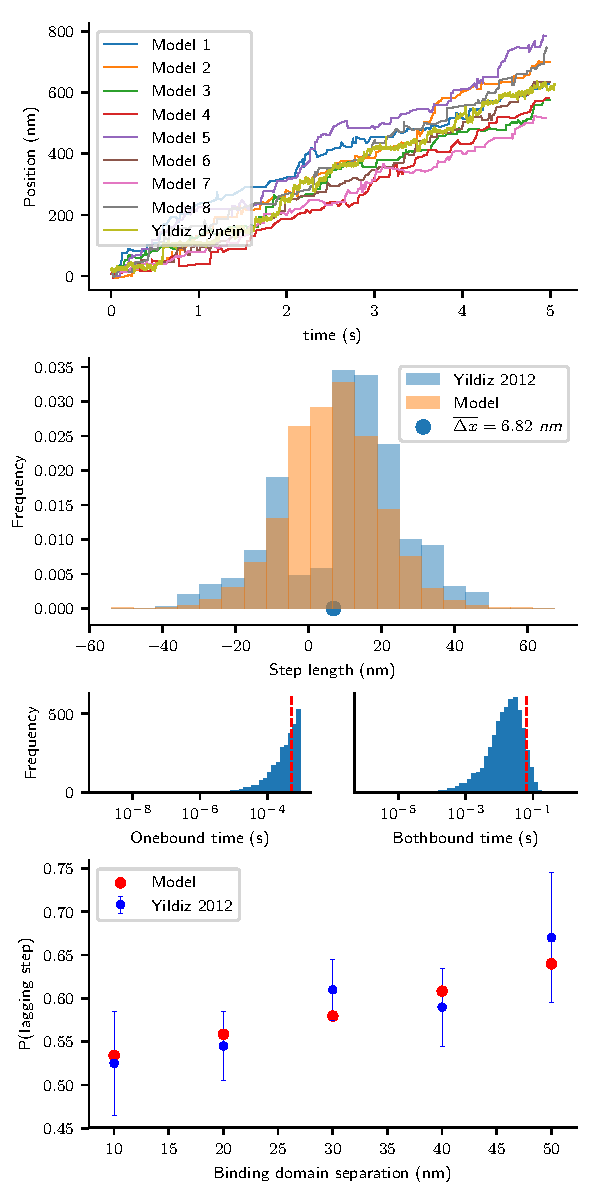
\includegraphics[width=\linewidth]{../../plots/paper_model_behavior}
  \includegraphics[width=\linewidth]{../../plots/paper_unbinding_probability_vs_L.pdf}
\caption{\textbf{Basic behavior of our model}}
\label{fig:}
\end{figure}

\begin{figure}[tbhp]
  \centering
  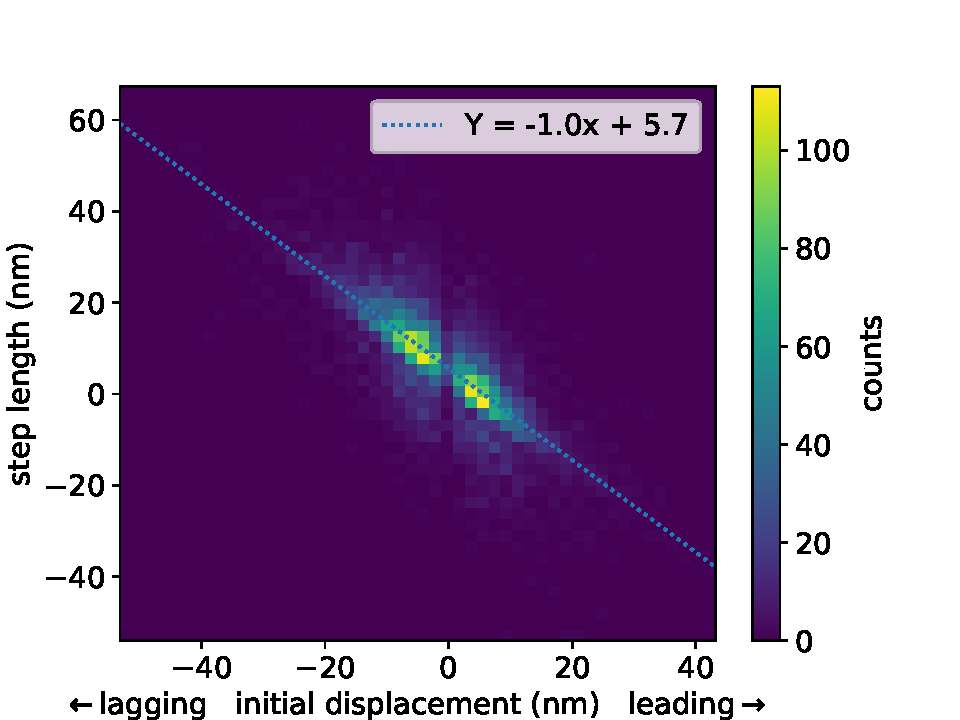
\includegraphics[width=\linewidth]{../../plots/paper_displacement_vs_step_length.pdf}
  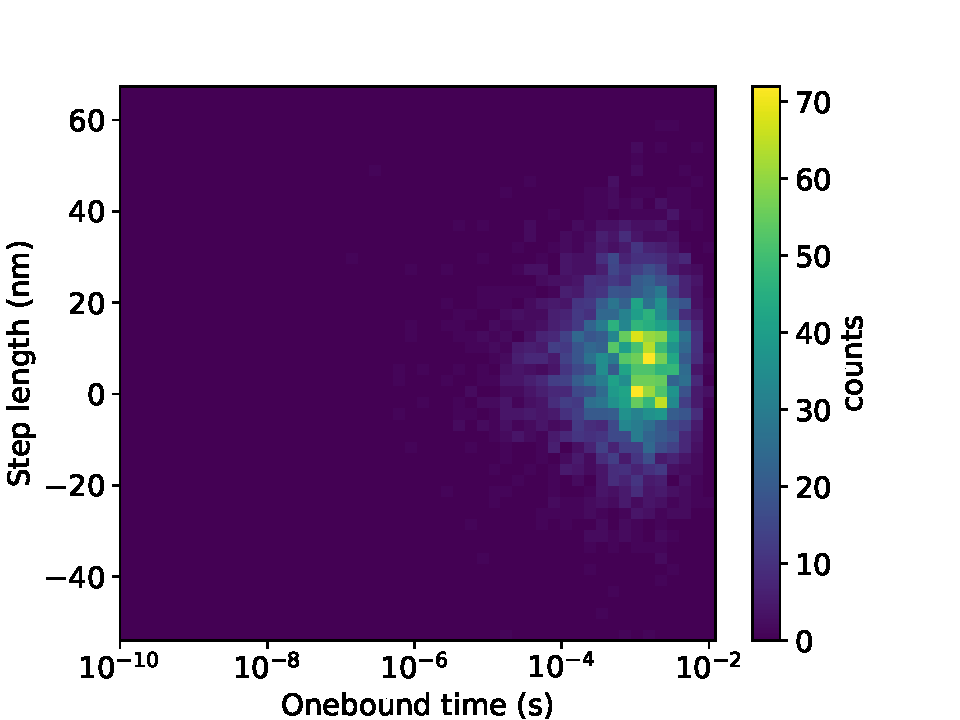
\includegraphics[width=\linewidth]{../../plots/paper_onebound_vs_steplength.pdf}
  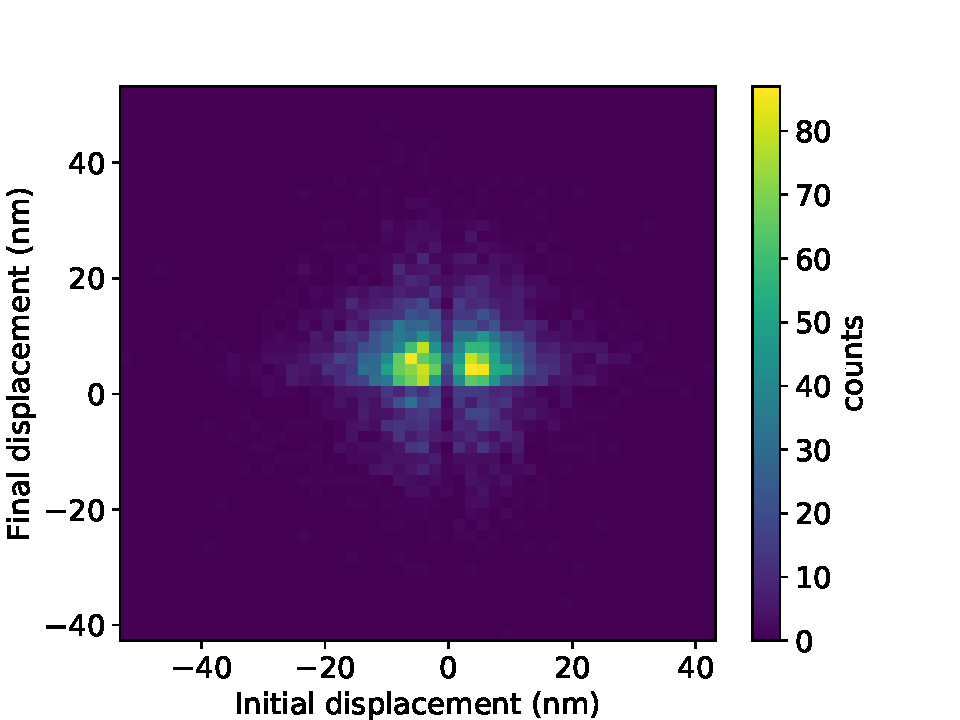
\includegraphics[width=\linewidth]{../../plots/paper_initial_vs_final_displacement.pdf}
\caption{\textbf{Does our model capture dynamics a markov model wouldn't?}}
\label{fig:}
\end{figure}

\begin{figure*}[tbhp]
    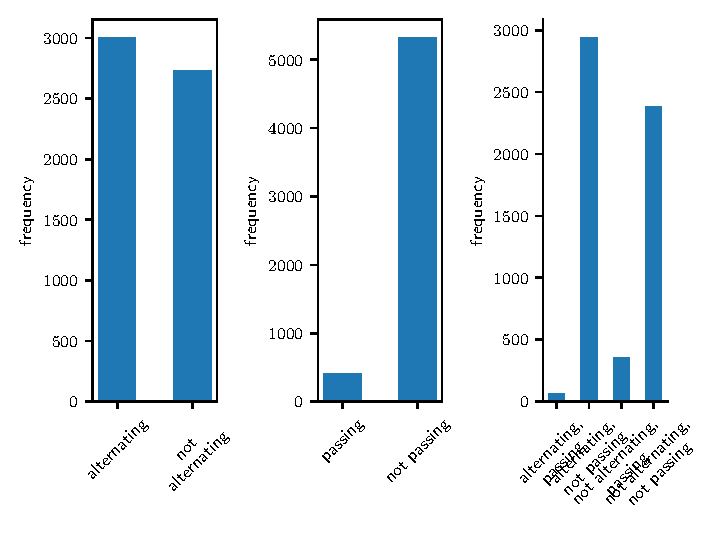
\includegraphics[width=0.5\linewidth]{../../plots/paper_foot_order_histogram.pdf}
\caption{The left plot is the $C=0$ case where the unbinding rate is
  independent of angle.  Here ``alternating'' means that the binding
  domain which did not move last time moved this time.  Passing means
  that the moving foot was behind, and ended up in front.}
\label{fig:steppingorder}
\end{figure*}

%% \begin{figure}[tbhp]
%%   \centering
%%    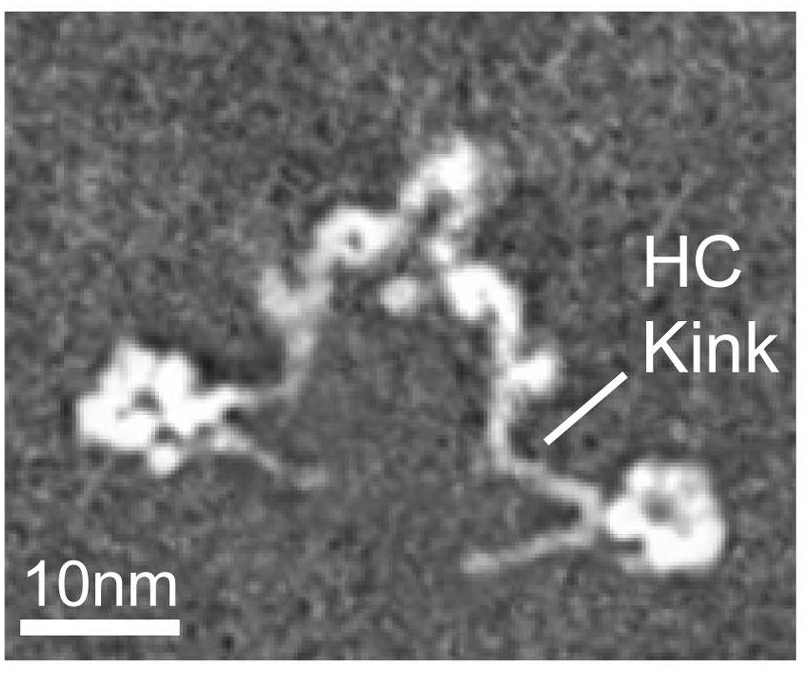
\includegraphics[width=0.3\columnwidth]{figures/schematic-1-cryoem}
%%    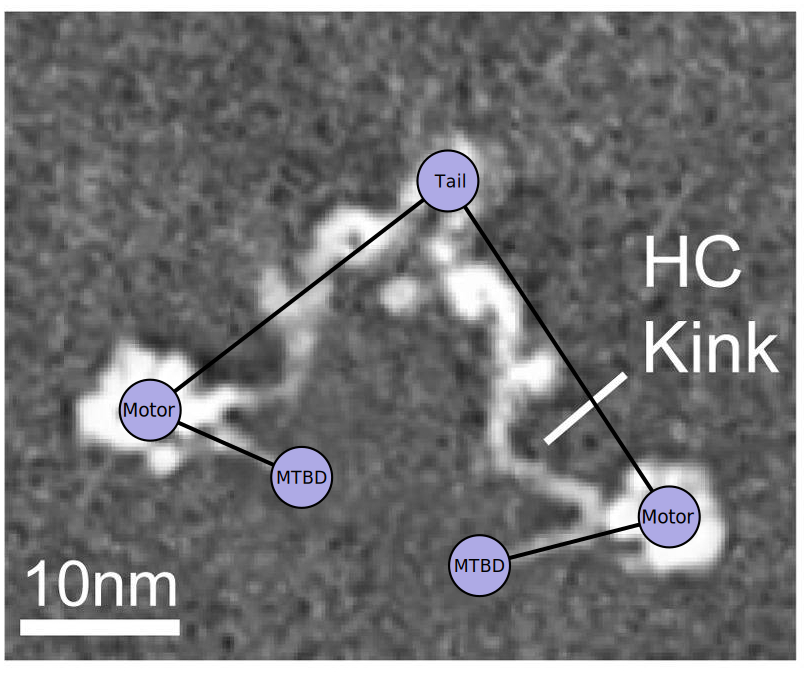
\includegraphics[width=0.3\columnwidth]{figures/schematic-1-superimposed}
%%    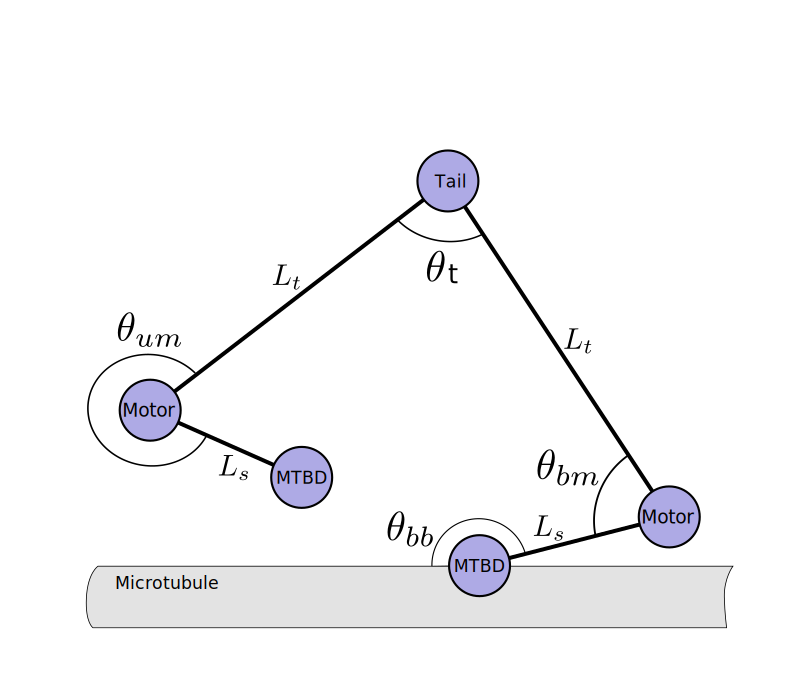
\includegraphics[width=0.3\columnwidth]{figures/schematic-1-model}

%%    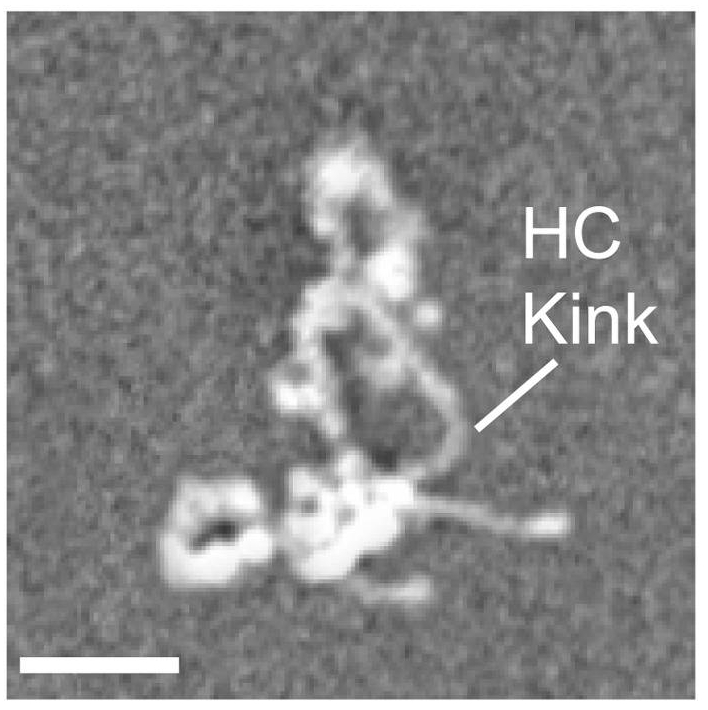
\includegraphics[width=0.3\columnwidth]{figures/schematic-2-cryoem}
%%    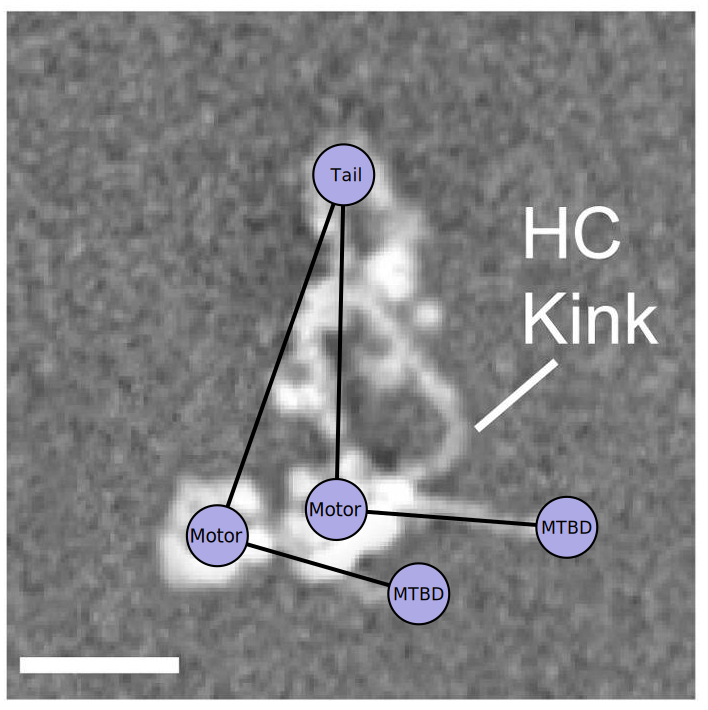
\includegraphics[width=0.3\columnwidth]{figures/schematic-2-superimposed}
%%    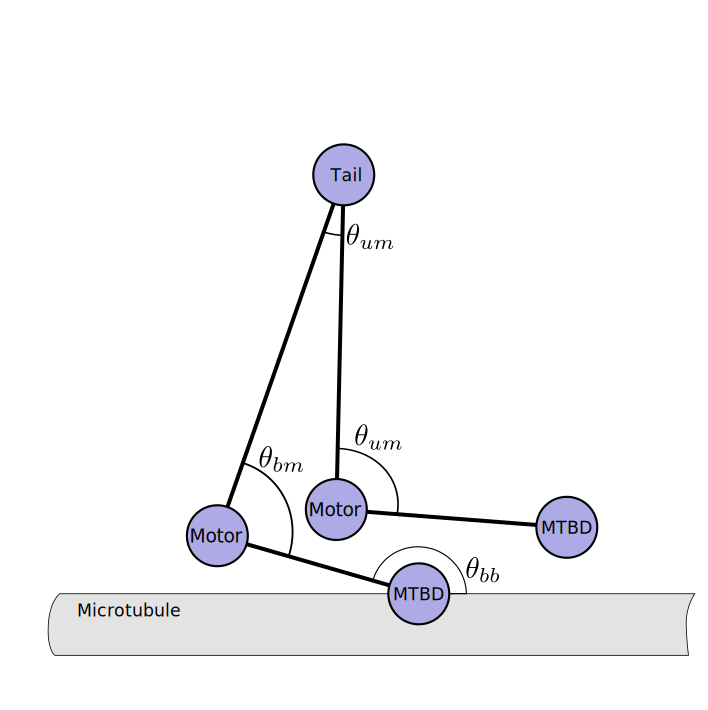
\includegraphics[width=0.3\columnwidth]{figures/schematic-2-model}
%%    \caption{\textbf{Model schematic superimposed on cryo-EM images of
%%        native dynein.} Native cryo-EM images of the full dimerized
%%      dynein complex composed of light, intermediate and heavy chains,
%%      from \cite{nativestructure}. Model schematics are superimposed
%%      for illustrative purpose; shown angles to not represent expected
%%      \textit{in vivo} equilibria. Schematics are shown docked to a
%%      microtubule for illustrative purposes.}
%%    \label{fig:modelparams}
%% \end{figure}

%% \begin{figure}[tbhp]
%%   \centering
%% 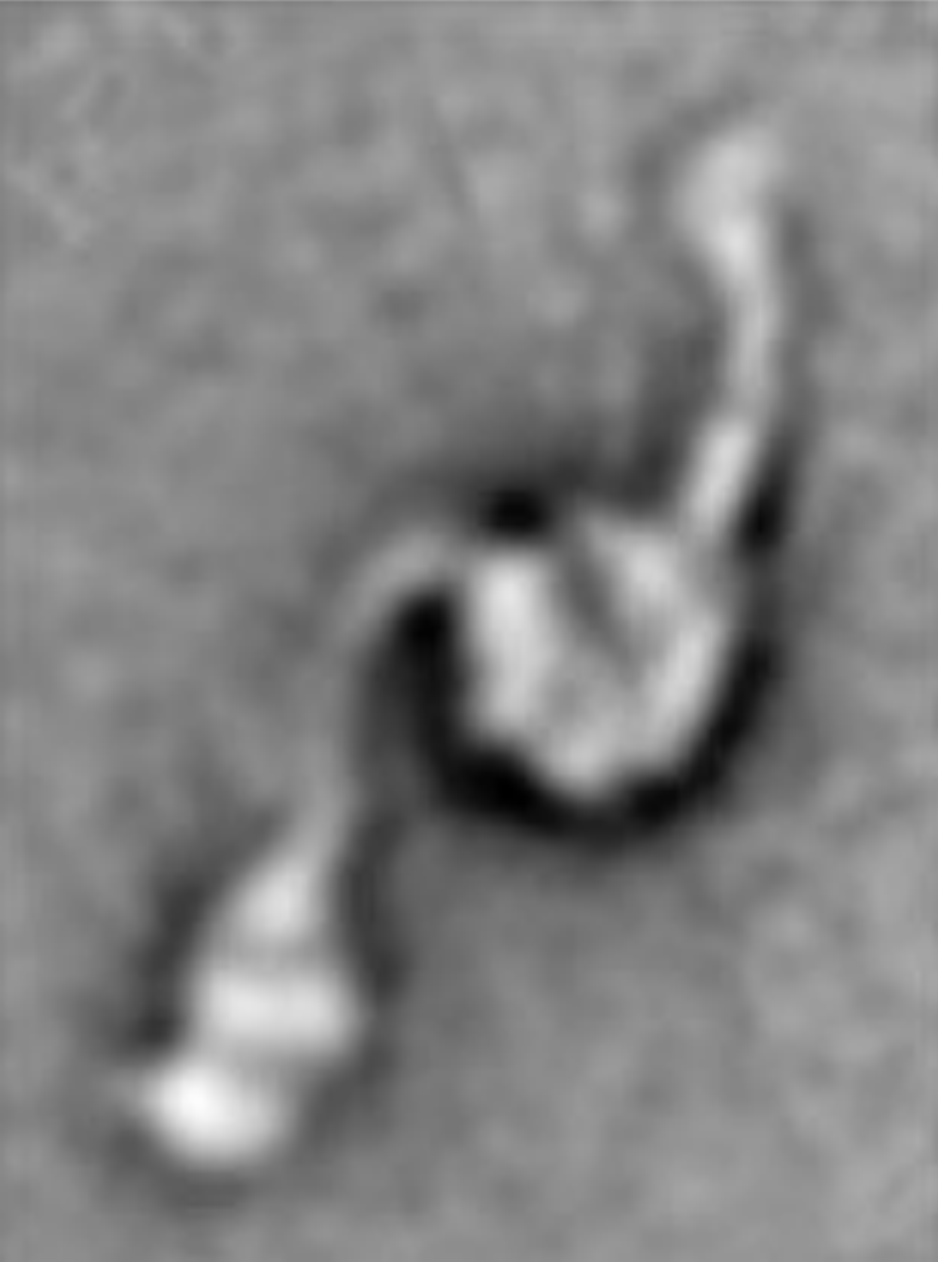
\includegraphics[width=0.5\columnwidth]{figures/schematic-prestroke}%
%% \includegraphics[width=0.5\columnwidth]{figures/schematic-poststroke}\\
%% \includegraphics[width=0.5\columnwidth]{figures/schematic-binding-angle}%
%% \includegraphics[width=0.5\columnwidth]{figures/schematic-full}
%%   \caption{\textbf{Schematic of model equilibrium angles over cryo-EM
%%       images.} \textbf{a.)} Prestroke and \textbf{b.)} poststroke
%%     dynein heavy chains superimposed with model motor angles, both
%%     from \cite{burgess-paper}. \textbf{c.)} Axonemal dynein bound to
%%     MT with model binding angle superimposed, from
%%     \cite{leschziner}. \textbf{d.} Full native dynein cryo-EM image
%%     bound to an MT with model superimposed, from
%%     \textbf{nativestructure}.}
%% \label{fig:modelangles}
%% \end{figure}

\begin{figure}[tbhp]
\centering
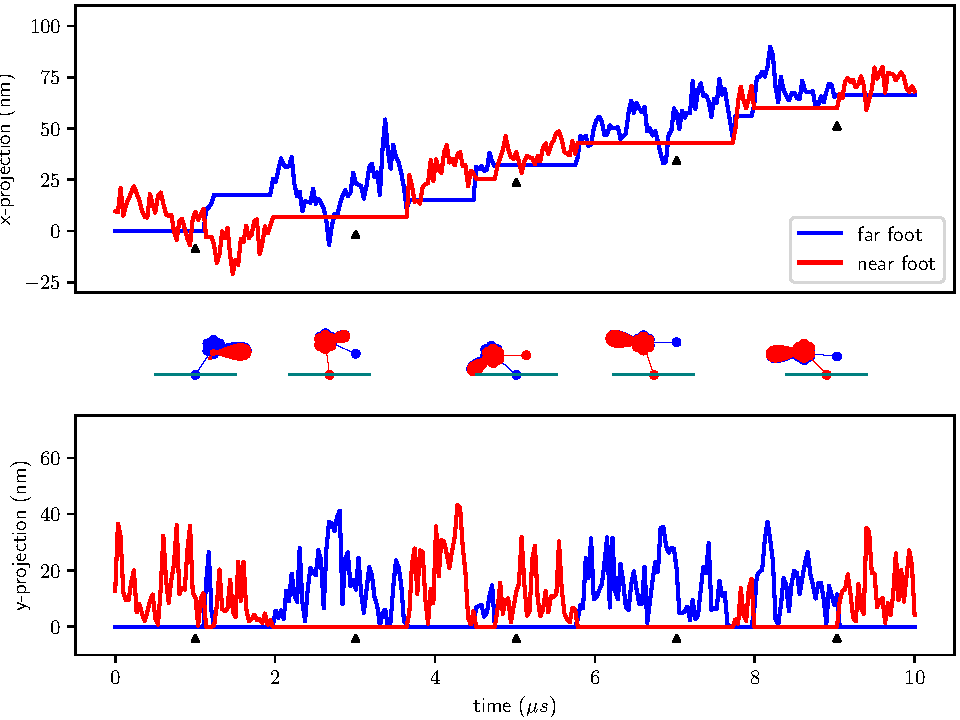
\includegraphics[width=\linewidth]{../../plots/paper_trajectory_plot.pdf}
\caption{\textbf{Model achieves forward-directed processivity.} \textit{Top view:} x-position of near and far binding domains during a 10 $\mu s$ simulation at high kinetic parameters of $k_b = \trajectorykb s^{-1}$ and $k_{ub} = \trajectorykub s^{-1}$. \textit{Middle view:} Cartoon snapshot of model at time indicated by bound binding domain. Teal lines correspond to the microtubule. \textit{Bottom view:} y-projection. Arrows on top and bottom plots correspond to respective snapshot times.}
\label{fig:trajectory}
\end{figure}

\section{To do items}

\subsection{Elliott}
\begin{enumerate}
\item Document carefully where all figures and data comes from.
\item Describe our algorithm in sufficient detail.
\item Fix stepping analysis python module to categorize zero-length
  steps separately from other steps, particularly in terms of stepping
  times.  Alternately, change C++ to make it possible to identify
  which foot lifted if it didn't move.
\item Update plotting scripts to use stepping analysis python module,
  or other modules.
\item Write up how we estimate one-bound/bothbound time ratio from
  processivity.  Ensure simulation obeys this?
\item Keep trying to get data from Yildiz.
\item Add force-dependent plots to compare with yildiz?
\end{enumerate}

\subsection{John}
\begin{enumerate}
\item Proofread the algorithm description, improve its writing, and
  check against code.
\item Figure out how to do no-unbinding simulations to get Yildiz
  comparison data.  Also this gives us unbinding rates that will agree
  with our stepping time, etc. \verb!src/simulate_unbinding_rates.cpp!
\item Play with parameters to get stepping length histogram more
  reasonable (this automatically gives us the velocity).
\item Run long/many simulations with final parameters.
\item Run a low-ATP simulation for comparison data.
\item Nice final version of stepping length histogram.
\item Nice final version of tension-gating Yildiz comparison.
\item Consider a no-binding simulation and a separable model.  Create
  a figure demonstrating/testing whether the histogram of final
  displacement is independent of initial displacement.
\item Consider a simple Monte Carlo that just uses our no-unbinding
  and no-binding simulations to model dynein (like Yildiz).
\end{enumerate}

\section{Papers we should cite}
This paper says something interesting~\cite{leschziner}.

% \pnasbreak splits and balances the columns before the references.
% If you see unexpected formatting errors, try commenting out this line
% as it can run into problems with floats and footnotes on the final page.
\pnasbreak

\bibliography{paper}

\end{document}
